
\section{Comparação SEIF vs Odometria}

Este primeiro experimento visa medir a capacidade do SEIF em estimar a 
pose do robô enquanto ele explora o ambiente de maneira autônoma, 
e compara essa estimativa 
com a odometria das rodas. Além disso, compara-se a estimativa do SEIF 
variando o cardinalidade do conjunto de \textit{landmarks} 
ativas $\{\bupvec{m}{+}\}$. O critério de comparação utilizado foi o 
Erro Absoluto Integral (IAE) (Equação \ref{eq:iae-error}) da posição estimada $\bvec{\hat{x}}$, em 
relação à pose real $\bvec{x}$ colhida do simulador. Para repetir o experimento com outro tamanho de $\{\bupvec{m}{+}\}$ foram gravadas a sequência de entradas $\bsubvec{u}{1:t}$ 
(posição angular das rodas) e a sequência de leituras $\bsubvec{y}{1:t}$ 
do sensor LiDAR.
\begin{equation}
  \IAE(\bvec{\hat{x}}, \bvec{x}) = \sum{
    \left\Vert \bsubvec{\hat{x}}{i} - \bsubvec{x}{i} \right\Vert_2
  }
  \label{eq:iae-error}
\end{equation}

A Tabela \ref{table:iae} lista os valores obtidos para o IAE. E a Figura \ref{fig:iae} ilustra a evolução 
temporal do erro da estimativa de posição do robô. Além 
da posição, também foi avaliado o erro na estimação da 
orientação, ilustrado na Figura \ref{fig:theta-error}. Em ambas as 
Figuras os valores obtidos pelo SEIF são mostrados separadamente pois na 
escala do erro da odometria eles aparecem sobrepostos.

\begin{table}[]
\caption{Erro Integral Absoluto da trajetória do robô para diferentes estimadores}
\label{table:iae}
\center
\begin{tabular}{cc}
\hline
Fonte da estimativa & $\IAE$ (m) \\ \hline
Odometria & 846.01 \\
SEIF $\bupvec{m}{+} = 4$ & \textbf{7.01 }\\
SEIF $\bupvec{m}{+} = 8$ & 8.04 \\ \hline
\end{tabular}
\end{table}

\begin{figure}
  \centering
  \begin{subfigure}{.75\textwidth}
    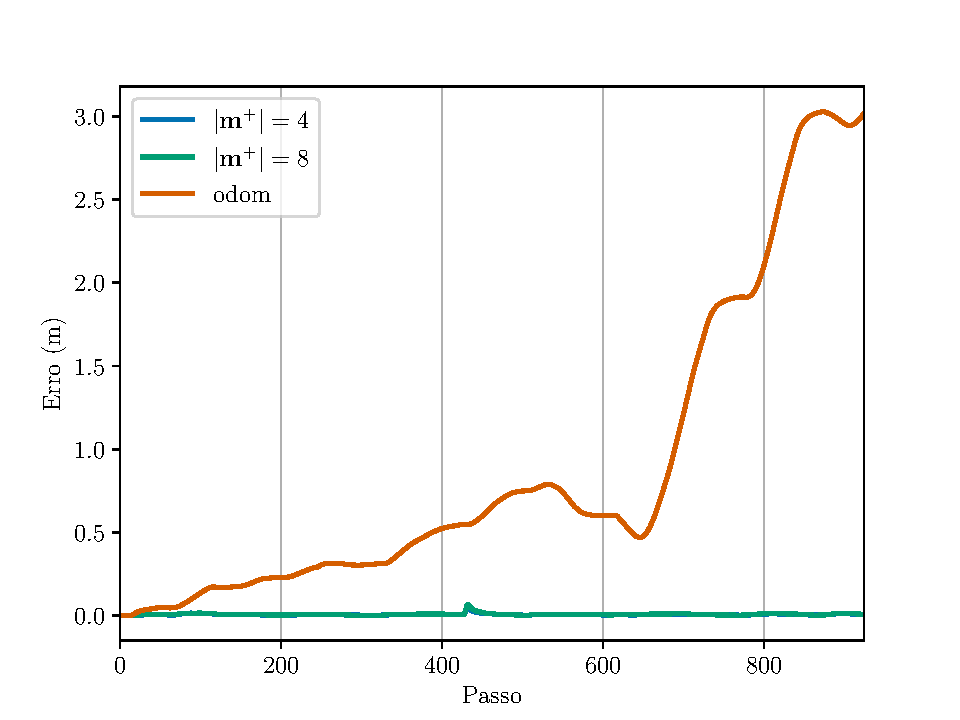
\includegraphics[width=\textwidth]{figs/iae-odom-seif.pdf} 
    \caption{Evolução temporal do erro da estimativa de posição pela odometria e das duas configurações do SEIF com $\lvert \bupvec{m}{+}\rvert = 4 $ e $\lvert \bupvec{m}{+}\rvert = 8 $.}
    \label{fig:iae-odom-and-seifs}
  \end{subfigure}
  \begin{subfigure}{.75\textwidth}
    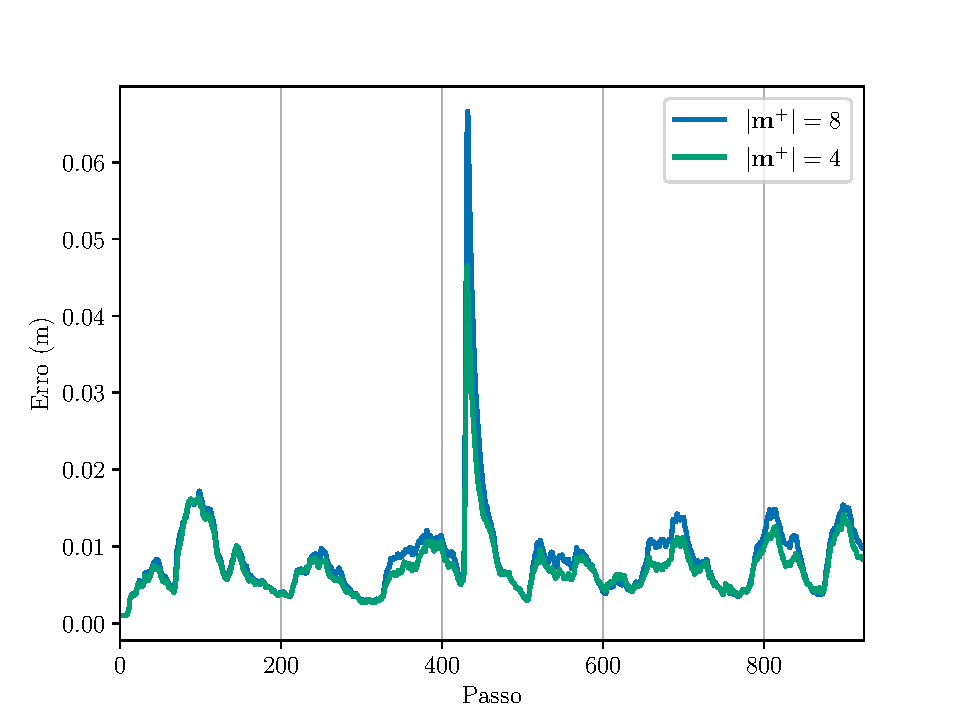
\includegraphics[width=\textwidth]{figs/iae-seifs.pdf} 
    \caption{Evolução temporal do erro da estimativa de posição das duas configurações do SEIF com $\lvert \bupvec{m}{+}\rvert = 4 $ e $\lvert \bupvec{m}{+}\rvert = 8 $.}
    \label{fig:iae-seifs}
  \end{subfigure}
  \caption{Erros de estimação da posição do robô durante exploração parcial do ambiente da Figura \ref{fig:environment}}
  \label{fig:iae}
\end{figure}

\begin{figure}
  \centering
  \begin{subfigure}{.75\textwidth}
    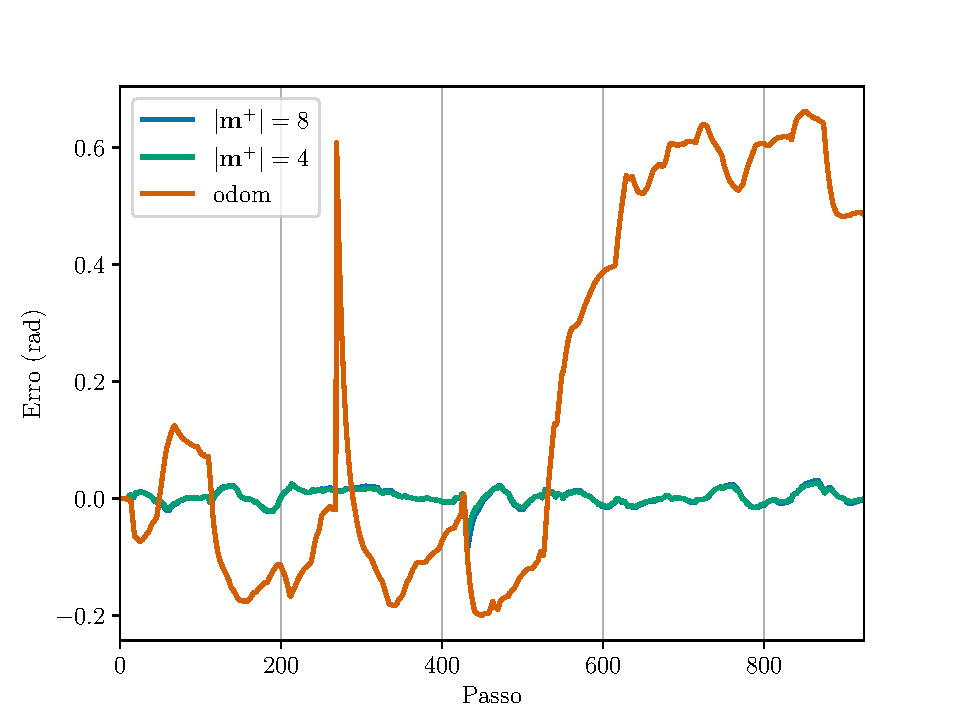
\includegraphics[width=\textwidth]{figs/theta-error-odom-seif.pdf} 
    \caption{Evolução temporal do erro da estimativa de orientação do robô pela odometria e pelas duas configurações do SEIF com $\lvert \bupvec{m}{+}\rvert = 4 $ e $\lvert \bupvec{m}{+}\rvert = 8 $.}
    \label{fig:theta-error-odom-and-seifs}
  \end{subfigure}
  \begin{subfigure}{.75\textwidth}
    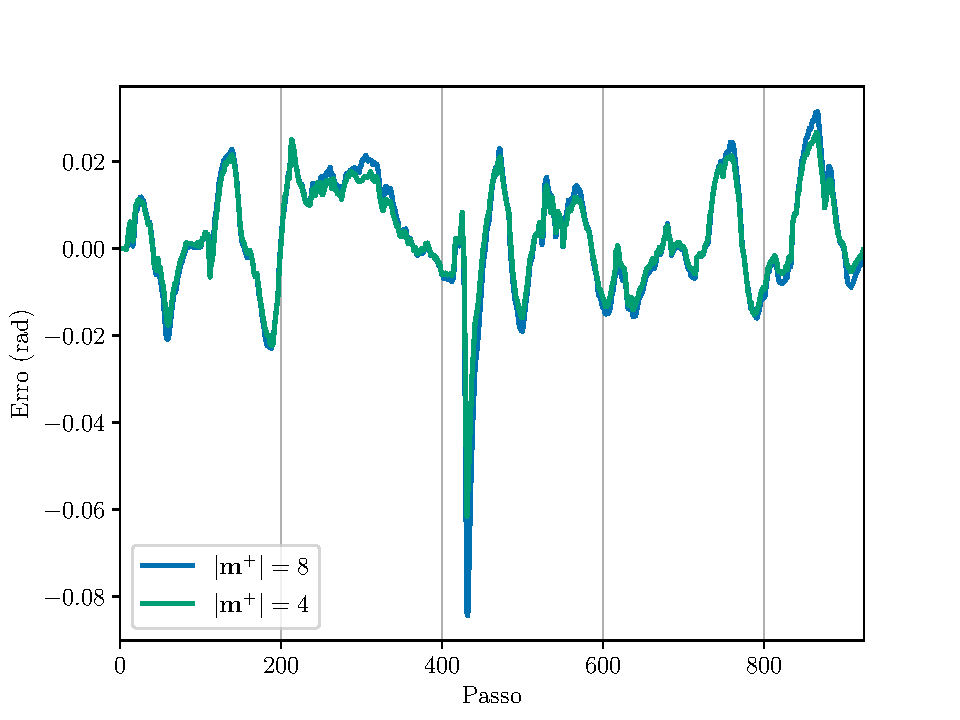
\includegraphics[width=\textwidth]{figs/theta-error-seifs.pdf} 
    \caption{Evolução temporal do erro da estimativa da orientação do robô pelas duas configurações do SEIF com $\lvert \bupvec{m}{+}\rvert = 4 $ e $\lvert \bupvec{m}{+}\rvert = 8 $.}
    \label{fig:theta-error-seifs}
  \end{subfigure}
  \caption{Erros de estimação da orientação do robô durante exploração parcial do ambiente da Figura \ref{fig:environment}}
  \label{fig:theta-error}
\end{figure}

Como esperado, ambas as configurações do SEIF estimaram 
de maneira satisfatória tanto a posição quanto a 
orientação do robô quando comparadas com a estimação da 
odometria. Porém, nota-se que a configuração com 
o cardinalidade do conjunto $\{\bupvec{m}{+}\}$ menor estimou 
melhor tanto a posição quanto a orientação, o que vai 
contra o consenso geral e a observação de \citeonline[p.~408]{bongard2006probabilistic} de que quanto maior o conjunto 
$\bupvec{m}{+}$ melhor é a estimativa. A causa dessa divergência não foi 
entendida até o momento da escrita deste texto.

\section{Comparações sobre uso de memória}
Neste experimento foram comparados o uso de memória de diferentes 
configurações do SEIF num mapa com 36 \textit{landmarks} e comparado com 
o uso que a abordagem mais clássica EKF-SLAM utilizaria. Nesse ensaio o 
robô foi teleoperado, e para garantir a reprodução exata do mesmo cenário 
as entradas e leituras foram novamente gravadas para alimentar as 
diferentes configurações do SEIF.

As quantidades de elementos não nulos da matriz de informação de cada 
parametrização estão compiladas na Tabela \ref{table:memory-usage}, e um 
comparativo com a quantidade de memória que seria utilizado pelo EKF-SLAM, 
com a mesma quantidade de \textit{landmarks}, é ilustrado na Figura \ref{fig:seif-memory-usage}. Por fim, as matrizes de informação são mostradas na 
Figura \ref{fig:seif-info-matrix-memory} para se ter uma uma ilustração de 
sua estrutura e quantidade e quantidade de elementos nulos, que não ocupam 
memória quando utilizada uma estrutura de dados adequada para a representação 
de matrizes esparsas.

O perfil de uso de memória observado mostrou-se como esperado, quanto maior 
o cardinalidade do conjunto de \textit{landmarks} ativas $\bupvec{m}{+}$, maior o 
consumo de memória pelo SEIF-SLAM. E além disso, todas as parametrizações 
muito menos memória quando comparados com o EKF-SLAM.

\newcolumntype{Y}{>{\centering\arraybackslash}X}
\begin{table}[]
\centering
\caption{Quantidade de elementos não nulos da matriz de informação esparsa para diferentes parametrizações do SEIF-SLAM}
\label{table:memory-usage}
\begin{tabularx}{\textwidth}{@{}YYY@{}}
\hline
cardinalidade do conjunto $\{\bupvec{m}{+}\}$ & Elementos não nulos da matriz de informação & 
Economia em relação ao EKF-SLAM\footnotemark{} \\ 
\hline
2 & 1721 & 69.40\% \\
4 & 1879 & 66.60 \\
8 & 2021 & 64.07\\
\hline
\end{tabularx}
\end{table}

\footnotetext{Embora esses valores correspondam ao número de elementos nulos em re relação ao tamanho total da matriz de informação, eles não representam necessariamente a economia de memória. Pois para que a a matriz esparsa seja representada é necessário utilizar memória extra para organizar o arranjo de armazenamento dos elementos. Porém, essa quantidade tende a ser irrisória quando comparada com a quantidade total de elementos de uma matriz densa. Na estrutura de dados utilizada nesse trabalho, a quantidade de memória utilizada para armazenas a matriz esparsa é da ordem de $\bigO{2n + N}$, onde $n$ é a quantidade de elementos não nulos e $N$ é a dimensão da matriz. Porém esses valores podem variar dependendo da técnica utilizada para armazenar a matriz.}

\begin{figure}
  \centering
  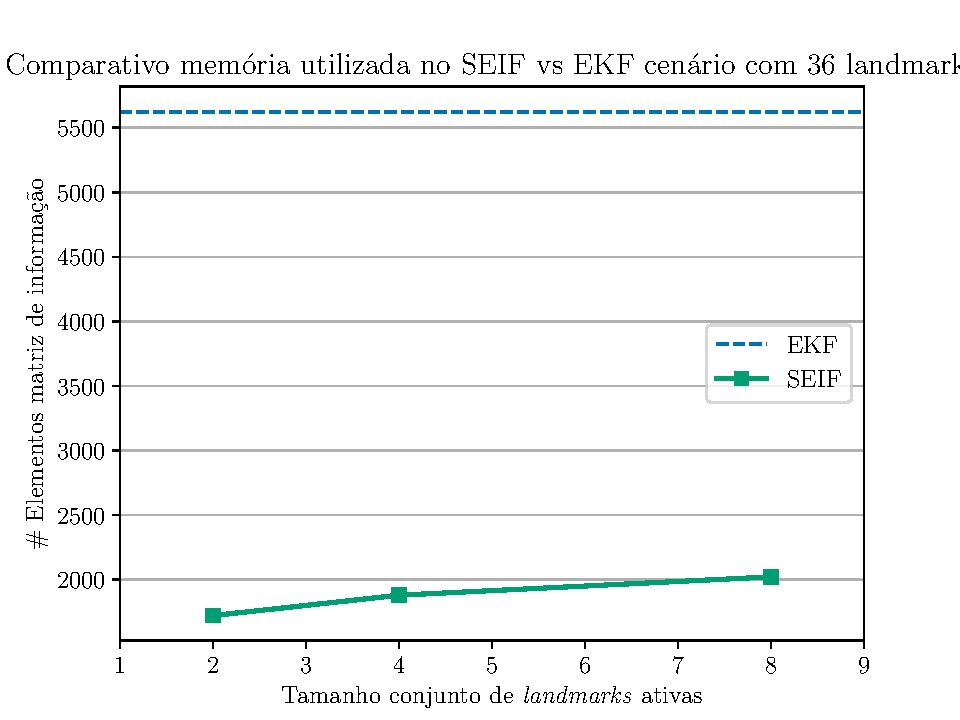
\includegraphics[width=0.7\textwidth]{figs/seif-memory-usage.pdf}
  \caption{Uso de memória para diferentes parametrizações do SEIF-SLAM com diferentes tamanhos (2, 4, 8) do conjunto de \textit{landmarks} ativas. A linha tracejada representa a quantidade de elementos quem a matriz do EKF-SLAM teria para o mesmo cenário.}
  \label{fig:seif-memory-usage}
\end{figure}

\begin{figure}
  \centering
  \begin{subfigure}{0.49\textwidth}
    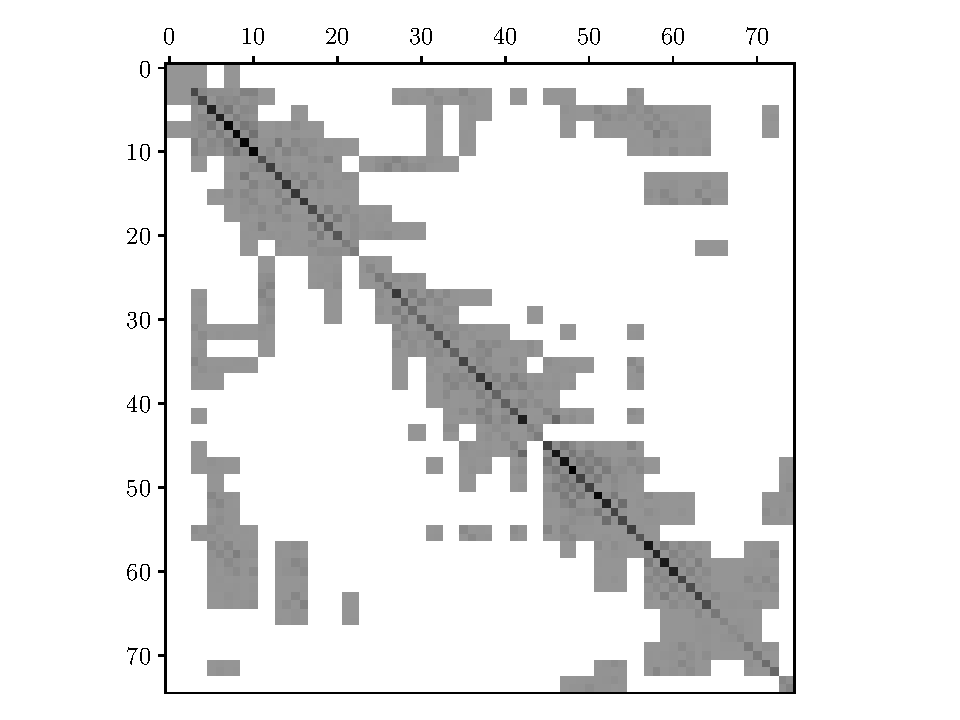
\includegraphics[width=\textwidth]{figs/seif-2-info-matrix.pdf} 
    \caption{$\lvert\{ \bupvec{m}{+} \}\rvert = 2$}
    \label{fig:seif-info-matrix-02}
  \end{subfigure}
  \hfill
  \begin{subfigure}{0.49\textwidth}
    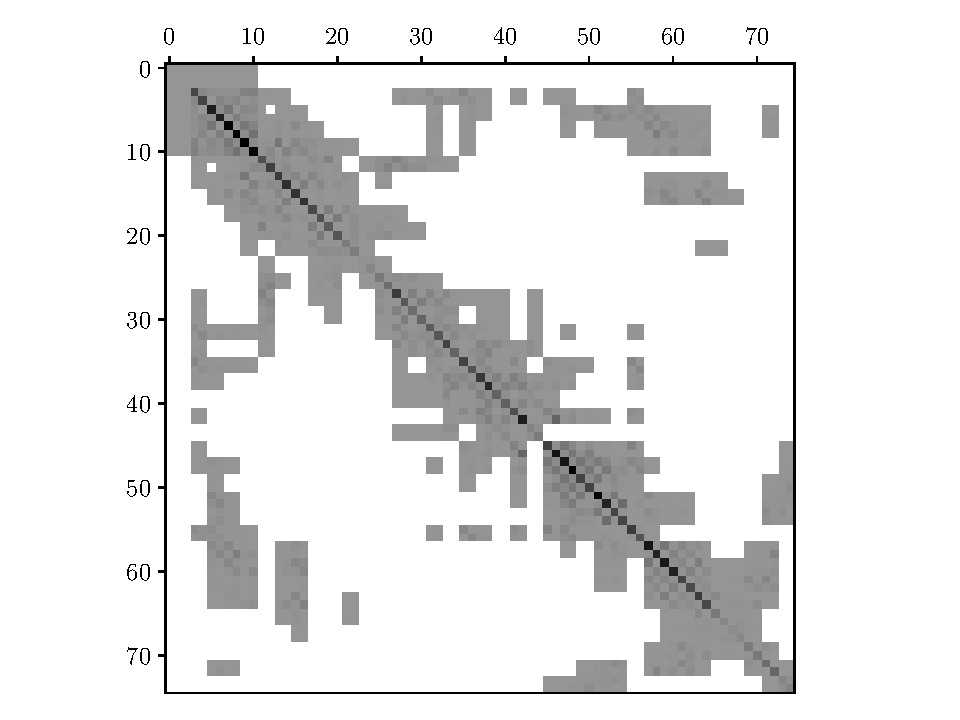
\includegraphics[width=\textwidth]{figs/seif-4-info-matrix.pdf} 
    \caption{$\lvert\{ \bupvec{m}{+} \}\rvert = 4$}
    \label{fig:seif-info-matrix-04}
  \end{subfigure}
  \begin{subfigure}{0.49\textwidth}
    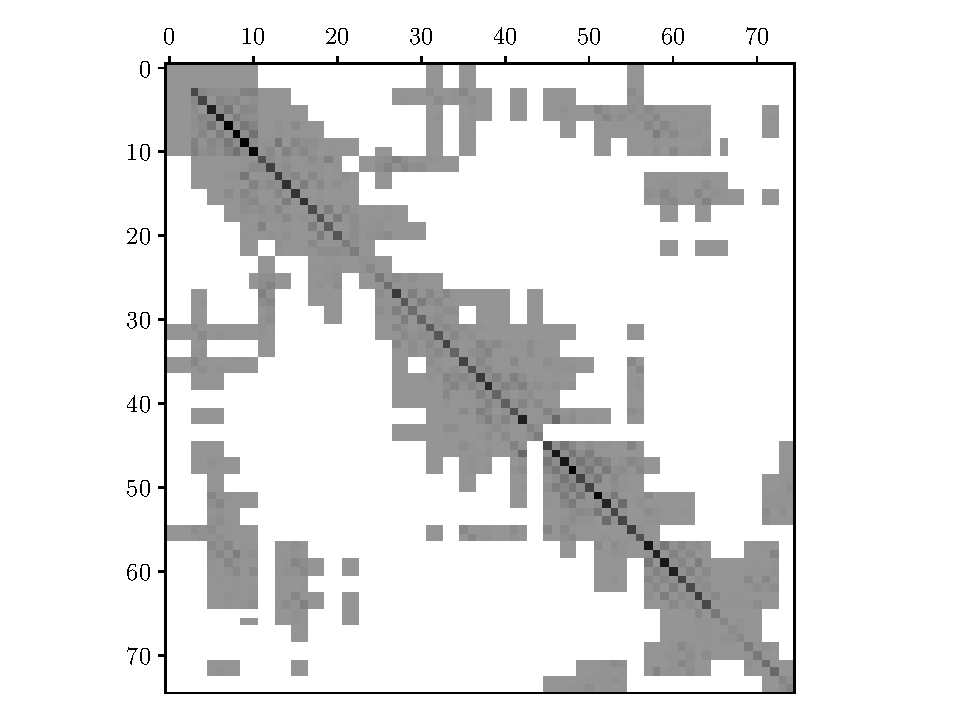
\includegraphics[width=\textwidth]{figs/seif-8-info-matrix.pdf} 
    \caption{$\lvert\{ \bupvec{m}{+} \}\rvert = 8$}
    \label{fig:seif-info-matrix-08}
  \end{subfigure}
  \caption{Representação das matrizes de informação correspondentes aos experimentos da Tabela \ref{table:memory-usage}. Os elementos nulos são representados pela cor branca, e os não nulos em escala de cinza. Quanto mais escuro o tom de cinza, maior a magnitude do valor representado.}
  \label{fig:seif-info-matrix-memory}
\end{figure}


\section{Mapeamento conjunto e descentralizado}
Esse experimento avalia cenários com mais de um robô desempenhando SLAM 
e trocando mapas entre sí como mostrado na Seção \ref{sec:seif-map-exchange}. Como tanto o vetor e matrix de informações 
quanto as grades de ocupação são compartilhados entre os agente, esse 
experimento é dividido em duas partes.

Na primeira o objetivo é medir a 
capacidade dos agentes de trocar os vetores e matrizes de informação 
entre sí (Seção \ref{sec:seif-info-exchange}) no cenário ideal onde a
transformação entre seus sistemas de referências é exata e conhecida, para isso são fornecidas as poses iniciais de cada agente. Enquanto que 
na segunda, os agentes não conhecem suas poses inicias e usam o 
registro de nuvem de pontos para calcular as transformações.

Nos cenários multiagente a comunicação ocorre sempre que dois robôs 
chegam a uma distância de dois metros um do outro e há um intervalo 
mínimo de 60 segundos entre duas comunicações consecutivas de um mesmo 
par de robôs. Erros de comunicação ou degeneração de mensagens não são 
simulados.

Para medir o desempenho de mapeamento dos robôs, 
calcula-se a área coberta 
por eles ao longo do tempo. A área coberta é definida como a soma das 
áreas de todas as células da grade de ocupação que possuem probabilidade 
de ocupação diferente de 50\%.

\subsection{Pose inicial conhecida}
\label{sec:exp-known-initial-pose}
Além do ganho de redundância, sistemas multiagentes também podem 
apresentar ganho de eficiência ao dividir a carga de trabalho entre os 
robôs. Para efeitos de comparação, primeiro foi realizado o mapeamento 
com apenas um robô, a curva da área coberta pelo tempo é ilustrada na 
Figura \ref{fig:area-coverage-single-robot}. Logo após o experimento foi repetido no mesmo ambiente com dois e três 
robôs, as curvas estão ilustradas na Figura \ref{fig:know-initial-pose-area-coverage}.

\begin{figure}
  \centering
  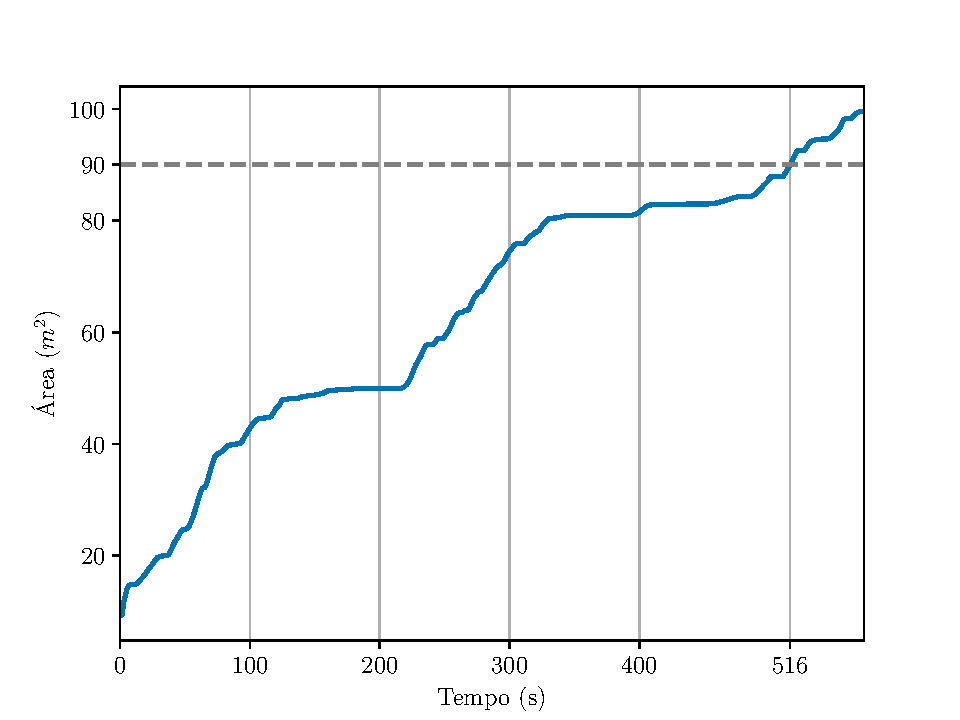
\includegraphics[width=.6\textwidth]{figs/area_coverage_single_robot.pdf}
  \caption{Evolução da área coberta ao longo do tempo por um único robô, 
  no ambiente representado na Figura \ref{fig:environment} com área total 
  de 100 $m^2$. O robô iniciou na posição $(2.5, 2.5)$, em relação ao centro do ambiente. Os platôs correspondem a intervalos nos quais o robô está atravessando uma área já mapeada para explorar uma nova fronteira.}
  \label{fig:area-coverage-single-robot}
\end{figure}

\begin{figure}
  \centering
  \begin{subfigure}{0.49\textwidth}
    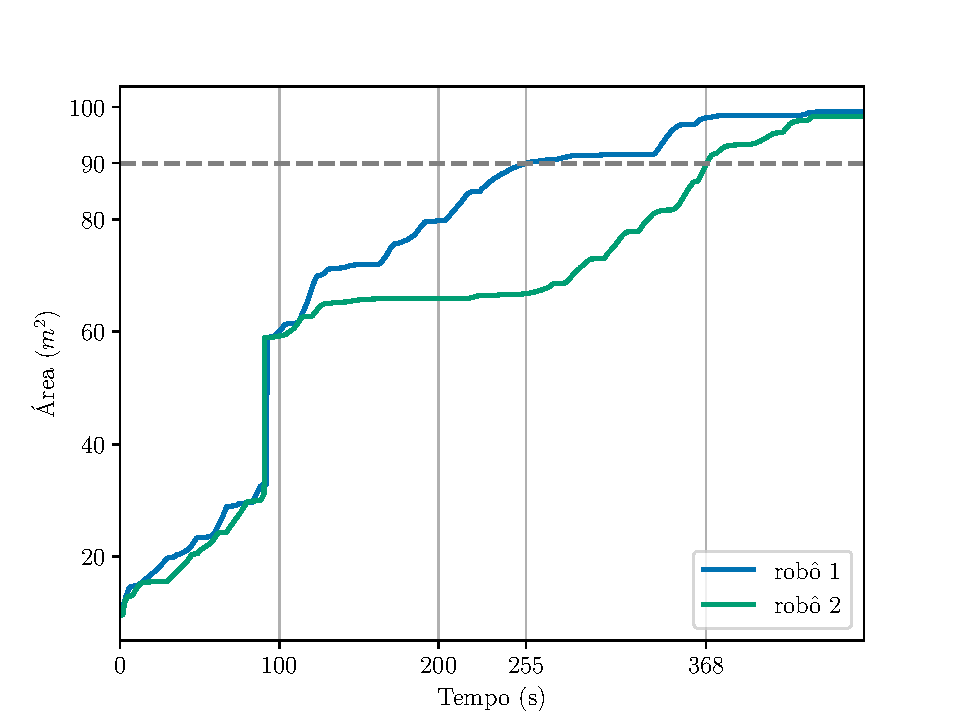
\includegraphics[width=\textwidth]{figs/area_coverage_two_robots-with-known-positions.pdf}
    \caption{Evolução da área coberta ao longo do tempo por dois robôs. 
    }
    \label{}
  \end{subfigure}
  \hfill
  \begin{subfigure}{0.49\textwidth}
    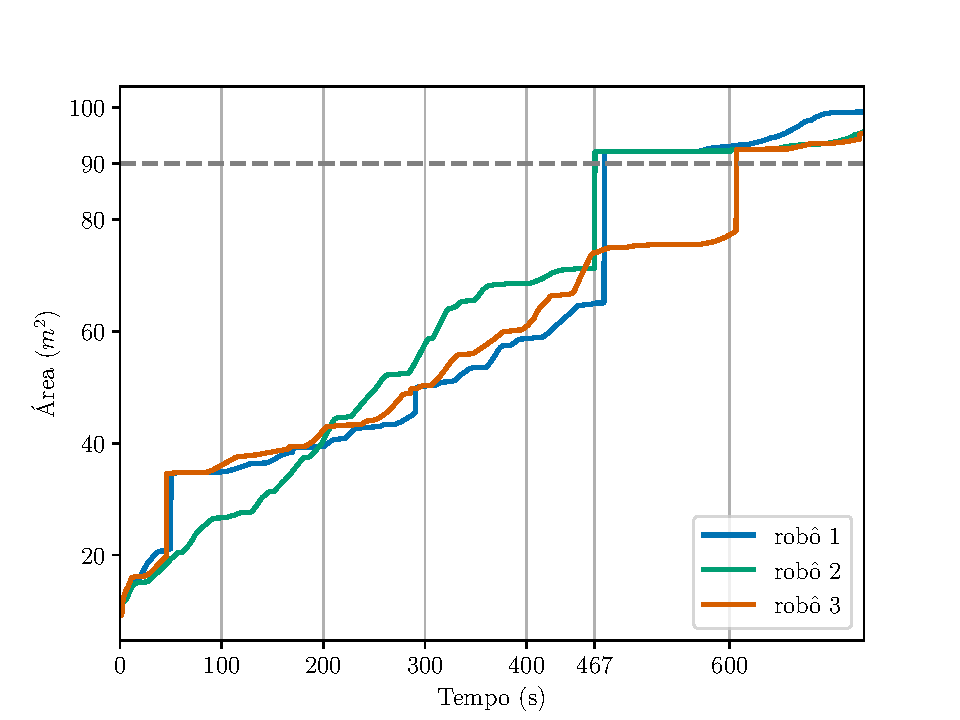
\includegraphics[width=\textwidth]{figs/area_coverage_three_robots-with-known-positions.pdf}
    \caption{Evolução da área coberta ao longo do tempo por três robôs. }
    \label{}
  \end{subfigure}
  \caption{Evolução da área coberta por dois e três agentes com pose inicial conhecida. Os momentos de comunicação e troca de mapas entre os agentes podem ser identificados por saltos verticais nas curvas de área coberta por cada agente.}
  \label{fig:know-initial-pose-area-coverage}
\end{figure}

A Tabela \ref{table:multiagent-exploration-know-initial-pose} registra o momento em que todos os agentes 
dos diferentes sistemas alcançam a marca de 90\% de área mapeada. Como é 
possível notar, quando houve ganho de eficiência ele não foi fez o tempo 
cair pela metade. E ainda no cenário com três robôs esse ganho foi negativo, o sistema levou mais tempo que o sistema com um único agente. 
Isso pode ser explicado por dois motivos: o primeiro é que não há uma 
política de exploração conjunta acordada entre os agentes, cada um 
explora o ambiente com base nas fronteiras presentes nos seus mapas 
individuais sem levar em consideração a posição de seus pares em relação 
a essas fronteiras; o segundo motivo é que a navegação se torna mais 
complexa pois agora um agente deve se desviar do outro durante a 
exploração e também não fazem isso de maneira sincronizada e/ou combinada.

\begin{table}[]
\center
\caption{Comparação entre o tempo levado para atingir a marca de 90\% de área coberta, de um ambiente de 100 $m^2$, entre os sistemas de múltiplos agentes e agente único.}
\label{table:multiagent-exploration-know-initial-pose}
\begin{tabularx}{\textwidth}{@{}YYY@{}}
\hline
Quantidade de agentes & Tempo para 90\% de área coberta (s) & Eficiência em relação a um agente \\ \hline
1 & 516 & - \\
2 & 368 & +40.21\% \\
3 & 600 & -14\% \\ \hline
\end{tabularx}
\end{table}

Apesar do ganho de eficiência geral dos sistemas ficarem abaixo do 
esperado, observando as Figuras \ref{fig:area-coverage-single-robot} e 
\ref{fig:know-initial-pose-area-coverage} é possível ver que o tempo 
levado pelo primeiro agente dos sistemas multiagentes para atingir a 
marca de 90\% de área coberta foi sempre menor que o tempo levado 
pelo sistema de agente único, com destaque para o sistema de dois agentes 
no qual o primeiro agente atingiu a marca em menos da metade do tempo 
do sistema de agente único.


\subsection{Pose inicial desconhecida}
\label{sec:exp-unknown-initial-pose}
Nesse último experimento, as poses iniciais dos agentes não foram 
fornecidas, como no experimento anterior. Dessa forma para incorporarem 
um o mapa do outro é necessário que calculem a transformação entre seus 
mapas de \textit{landmarks} utilizando a técnica de registro de nuvem de 
pontos discutida na Seção \ref{sec:point-cloud-registration}. A Figura 
\ref{fig:unknown-initial-pose-area-coverage} mostra duas execuções do 
sistema SLAM com dois robôs, entre elas variou-se apenas as posições 
iniciais dos agentes.

\begin{figure}
  \centering
  \begin{subfigure}{0.49\textwidth}
    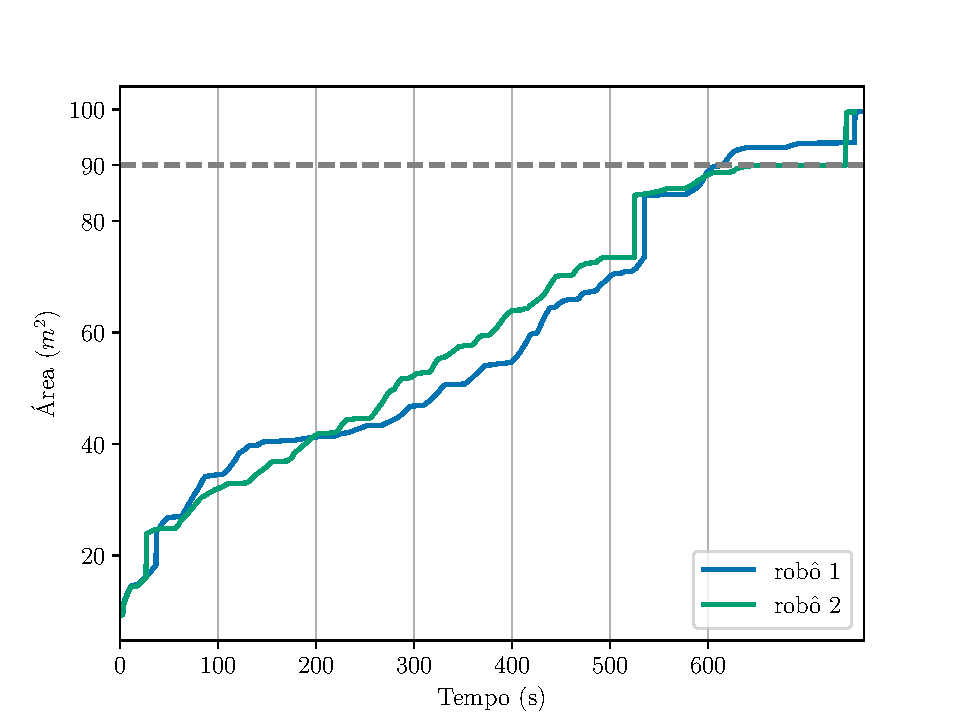
\includegraphics[width=\textwidth]{figs/area_coverage_two_robots-with-unknown-positions-01.pdf}
    \caption{}
    \label{fig:unk-pose-area-coverage-first}
  \end{subfigure}
  \hfill
  \begin{subfigure}{0.49\textwidth}
    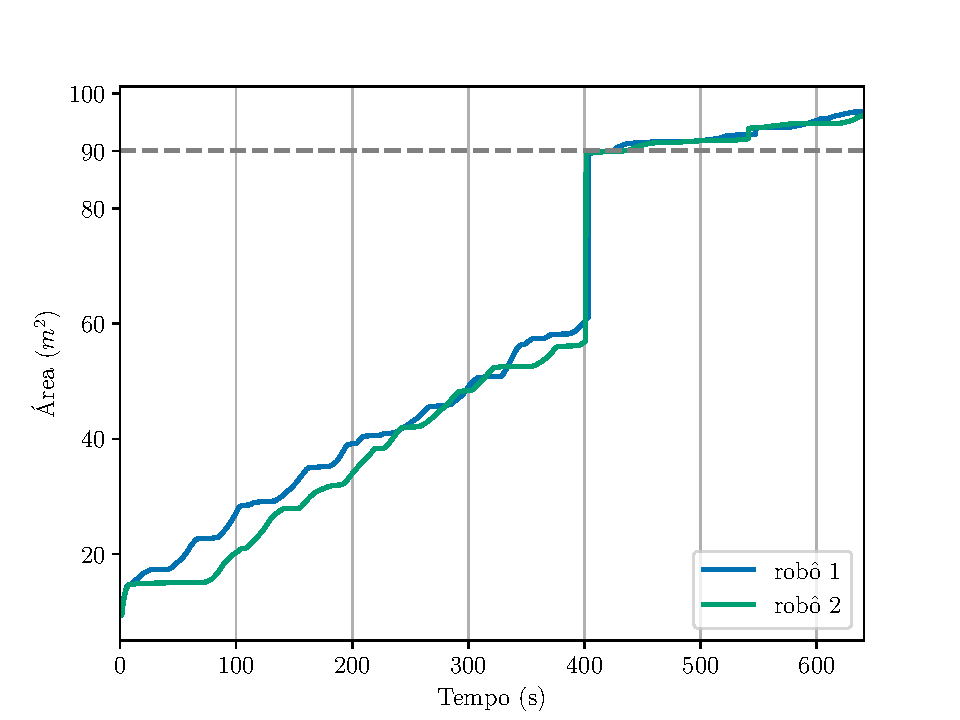
\includegraphics[width=\textwidth]{figs/area_coverage_two_robots-with-unknown-positions-02.pdf}
    \caption{}
    \label{fig:}
  \end{subfigure}
  \caption{Diferentes execuções do mapeamento com dois agentes com pose inicial desconhecida. Entre as execuções variou-se a pose inicial dos 
  agentes. As curvas da Figura da direta estão defasadas pois o segundo 
  agente foi colocado no ambiente alguns instantes depois que o primeiro.}
  \label{fig:unknown-initial-pose-area-coverage}
\end{figure}

Além dos problemas de sincronia entre os agentes, já citados no experimento 
anterior, neste exemplo também foram observados problemas com a estimação 
da transformação entre os mapas de \textit{landmarks} dos agentes. 
Enquanto no experimento anterior a troca de mapas entre os robôs sempre 
ocorre com sucesso, pois eles sabem suas poses iniciais e portanto sabem 
relacionar o mapa de um com o do outro. Neste nem toda aproximação dos 
robôs resultou em troca dos mapas, pois muitas vezes eles não conseguiram 
estimar a transformação entre os mapas.

Este experimento também teve que ser repetido mais de uma vez, pois em 
algumas execuções os robôs estimavam a transformação errada, incorporando 
a informação do outro de maneira errada e provocando divergência do 
filtro. Desse modo a técnica de registro de nuvem de pontos utilizada 
se mostrou capaz de calcular a transformação entre os mapas dos robôs, 
mas não se mostrou robusta e confiável.

